\documentclass{beamer}
\usepackage{listings}
\lstset{
%language=C,
frame=single, 
breaklines=true,
columns=fullflexible
}
\usepackage{subcaption}
\usepackage{url}
\usepackage{tikz}
\usepackage{pgfplots}
\pgfplotsset{compat=1.17}
\usepackage{tkz-fct}
\usepackage{mathrsfs}
\usepackage{txfonts}
\usepackage{tkz-euclide} 
\usetikzlibrary{calc,math}
\usepackage{float} 
\newcommand\norm[1]{\left\lVert#1\right\rVert}
\renewcommand{\vec}[1]{\mathbf{#1}}
\usepackage[export]{adjustbox}
\usepackage[utf8]{inputenc}
\usepackage{amsmath}
\usetheme{Boadilla}
\title{Research Paper Presentation}
\author{ARUN SIDDARDHA - AI20BTECH11019}
\begin{document}
\begin{frame}
\titlepage
\end{frame}
\section{}
\begin{frame}
    \begin{block}{Title}
   Recommendations in the social network using the link prediction technique
    \end{block}
    \begin{block}{Authors}
    \begin{itemize}
        \item Ramya BV , Assistant professor, Departmnet of ISE
        \item Dr.N Sandeep Varma ,Assistant professor, Departmnet of ISE
        \item R Indra ,Assistant professor, Departmnet of ISE
    \end{itemize}
    \end{block}
\end{frame}
\begin{frame}
\begin{block}{Abstract}
\begin{enumerate}
    \item Currently social media is getting developed rapidly and it has become a part of peoples life.Based on user interest social network will also change over time with different nodes and edges.
    \item New relations can be predicted between nodes in social network by link prediction technique.This can be done by creating a machine learning model which estimates the probabilities of the new connection /relation that are going to be possible in future with the given data set.
    \item We will talk about steps followed in building the model and discuss about the steps involved.Then Find the best features and best classifiers for effectively building the model.Which predicts the connections with high probability and accuracy.
\end{enumerate}
\end{block}
\end{frame}
\section{Introduction}
\begin{frame}{Building machine learning model}
For building a machine learning model for prediction the following steps are followed 
\begin{enumerate}
    \item Data collection
    \item Data preprocessing
    \item Feature engineering
    \item Test-train-split
    \item Building classifier
    \item Evaluation
\end{enumerate}
\end{frame}
\begin{frame}{Explanation}
\begin{block}{Data collection}
 A large amount of data is collected from social network as nodes and edges.Where nodes represent the users and the edges represent the friendship of the users.
\end{block}
\begin{block}{Data preprocessing}
 After the data is collected edges are assigned class labels.An edge is termed as a missing edge if the shortest distance from the source node and the destination node is more than 2.Because if the shortest distance is less than 2 then there will be probability of them getting connected in future. By considering this class label 1(positive) is given for the already present edges and class label 0(negative) for the missing edges.
\end{block}
\end{frame}
\begin{frame}{Feature engineering}
From the collected Dataset different features are extracted and from them top 10 features are selected by doing the chi-Square test on that features.Given below are some features.
\begin{block}{Jaccard similarity index}
It calculates the similarity between the node pairs.
$$Jaccard(p,q)=\frac{N_{p}\cap N_{q}}{N_{p}\cup N_{q}}$$
$N_{p}$ and $N_{q}$ represent neighbours of node p and q respectively
\end{block}
\begin{block}{Cosine similarity index}
It measures similarity with the cosine of the angle between vectors which is pointing in same direction.mathematical representation.
$$cosine(p,q)=\frac{N_{p}\cap N_{q}}{\sqrt{N_{p}*N_{q}}}$$
\end{block}
\end{frame}
\begin{frame}
\begin{block}{Frequency weighted common neighbour}
In this smaller degree of the common neighbours are weighted heavily.
$$AA(p,q)=\sum_{z \in (N_{p}\cap N_{q})}1/log(N_{z})$$
\end{block}
\begin{block}{Page rank}
It is used to measure the connectivity of nodes based on the in-degree of the node and it computes the ranking. Where page rank is used for both followers and followees.
here O(j) represents outer links of the node j. 
$$Pagerank(i)=\sum_{(j,i)\in E}\frac{P(j)}{O(j)}$$
\end{block}
\end{frame}
\begin{frame}
\begin{block}{Weakly Connected Components}
It calculates all path 
between nodes without considering the direction.
\end{block}
\begin{block}{Follow back}
If the source node is following the destination node and destination node is also following to source node then that nodes are added in this feature.
\end{block}
\begin{block}{Inter Followers and Followee Count}
It represents a number of common followers and followees between the source and destination node.
\end{block}
\begin{block}{Follower and Followee Counts}
The intuition of this feature is 
popular streamer has a greater number of followers and can be recommended for users.It is used to the calculated 
total number of followers and the total number of followees of source and destination node.
\end{block}
\end{frame}
\begin{frame}
    \begin{block}{Shortest path}
    Here, intuition is the shortest distance between nodes have a high probability of connecting in future so it can be used for recommendation.
    \end{block}
    \begin{block}{Katz}
    It calculates all the paths between node pair with assigning a high score to the shortest path and low value to a longer path. It uses a factor of $\beta$ to calculate values and mathematically represented as
    $$Katz\left(p,q\right)=\sum_{l=1}^{\infty}\beta^{l}\mid paths_{p,q}^{<l>}\mid$$ 
    \end{block}
\end{frame}
\begin{frame}{Chi-square test}
It measures the deviation between observed count and expected count for all features. 
$$x^{2}=\sum \frac{(O-E)^{2}}{E}$$
O is the observed value and E is the expected value.
By using this top 10 scores are extracted for the features and shown in the below graph
\begin{figure}[ht]
    \centering
    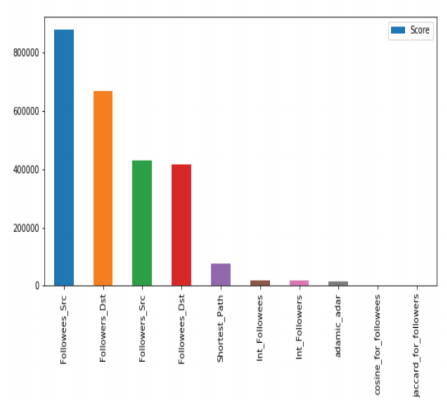
\includegraphics[width =0.5\columnwidth]{chi-square.png}
\end{figure}
    
\end{frame}
\begin{frame}{Test-train split}
In machine learning dataset as to be split into train and test 
data. Where train data is used to train the model and model is 
tested with test data to measure the model performance.
so 70\% data is splitted into  test and 30\% to training data.Model has to be trained by the training data and tested with testing data.if machine is tested with the measure accuracy of the model goes wrong.
\end{frame}
\begin{frame}{BUILDING CLASSIFIERS}
The most important part is to build a classifier which classifies the Data accurately.For that here supervised machine learning is used where the model is trained to classify the labes 1 and 0 into sepearate parts.Give below are types of algorithms 
\begin{block}{Logistic regression classifier}
It is the technique for the analysis where it measures relation between dependent variables which is lables and independent variables (features used).Probability of prediction is calculated by below formula.
$$G(X)=ln  \left[\frac{p(X)}{1-p(X)}\right]=\beta_{0}+\beta_{1}X$$
\end{block}
\end{frame}
\begin{frame}
    \begin{block}{Bagging classfier}
It is one of the classifier where  prediction is calculated by aggregating individual prediction to reduce variance .Here dataset is divide into different samples and trained. Bagging classifier for decision tree is implemented with a majority vote and 
mathematical formula used as below
$$f(X)=sign\left(\sum_{i=1}^{T}sign(f_{i(x)})\right)$$
\end{block}
\begin{block}{XGBoost}
It is the highly scalable , quick to execute algorithm.XGBoost refers to Extreme Gradient Boosting which is efficient for building a classification model and it is boosting algorithm which uses gradient boosting framework. 
\end{block}
\end{frame}
\begin{frame}{Evaluation}
After building the model it is important to train the model with training data and test it with the test data.After that is over now it is important to measure the performance of the model.This can be done using the following performance metrics.
\begin{block}{Confusion matrix}
It is used to find the correctness and accuracy of the model.it is represented as below.\\
\begin{figure}[ht]
    \centering
    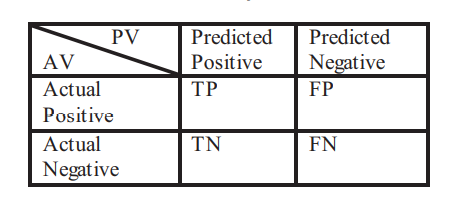
\includegraphics[width =0.5\columnwidth]{confusion matrix.png}
\end{figure}
\end{block}
\end{frame}
\begin{frame}
\begin{block}{Notation}
\textbf{TP(true positive)}:\\The samples correctly predicted as future links. Edge present between nodes is Positive (1),
classified correctly as positive (1).\\
\textbf{TN (True negative)}:\\ The samples correctly not predicted as future links. No edges between nodes is Negative
(0),correctly classified Negative (0).\\
\textbf{FP (False Positive)}:\\ The samples
incorrectly predicted as future links
Positive (1) edges are misclassified as
negative\\
\textbf{FN (False negative)}:\\ The samples incorrectly not predicted as future links. Negative (0) edges are misclassified as Positive (1) edge

\end{block}
\end{frame}
\begin{frame}
\begin{block}{ROC Curve}
It is used for the binary classification model .It plots true positive rate vs false positive rate for various threshold values.
and they are calculated as.
$$TPR = \frac{number\;of\;correctly predicted \;future \;links}{number\; of \;the\; actual\;future \;links}$$

$$FPR = \frac{number\;of\;incorrectly\; predicted \;future \;links}{number\;of \;the \;actual\; negative\; links}$$
\end{block}
\begin{block}{Precision-recall}
It is a plot between precision and recall. The high area under curve obtained from Precision-Recall curve represents high precision and high recall.
$$precision=\frac{TP}{TP+FP}$$
$$recall=\frac{TP}{TP+FN}$$
\end{block}
    
\end{frame}
\begin{frame}{EXPERIMENTS AND RESULTS}
Data set is collected and the data is taken through the above process using the different  data models  algorithms such as logistic regression,XGBoost,Bagging classifier.And they are evaluated based on the given performance metrics. And the accuracy, precision and quality of the models is found.
\begin{figure}[ht]
    \centering
    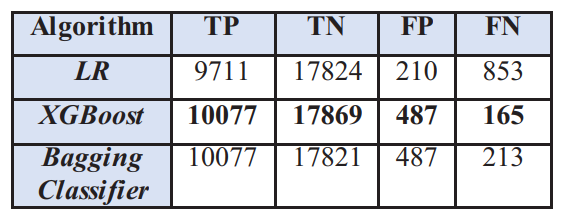
\includegraphics[width =0.7\columnwidth]{experiment matrix.png}
\end{figure}
From the confusion matrix obtained for different classifiers highest value of TP and TN is obtained using XGBoost algorithm.
Using the performance values TP,TN,FP,FN the ROC curves and precision-recall curves are plotted.
\end{frame}
\begin{frame}
\begin{block}{ROC plot}
\begin{figure}[ht]
  \subfloat[\scriptsize{logistic regression}]{
	\begin{minipage}[c][1\width]{
	   0.3\textwidth}
	   \centering
	   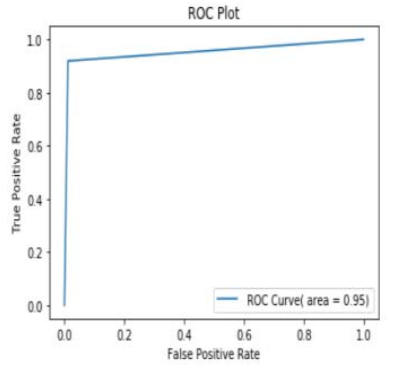
\includegraphics[width=1\textwidth]{Roc logistic.png}
	\end{minipage}}
 \hfill 	
  \subfloat[\scriptsize{XGBoost}]{
	\begin{minipage}[c][1\width]{
	   0.3\textwidth}
	   \centering
	   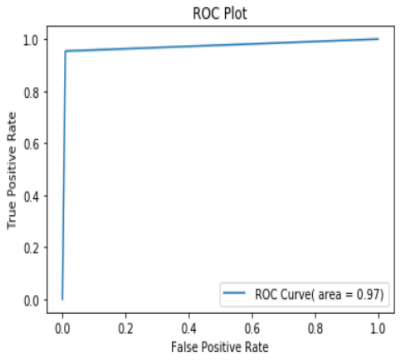
\includegraphics[width=1\textwidth]{Roc XGBoost.png}
	\end{minipage}}
 \hfill	
  \subfloat[\scriptsize{Bagging}]{
	\begin{minipage}[c][1\width]{
	   0.3\textwidth}
	   \centering
	   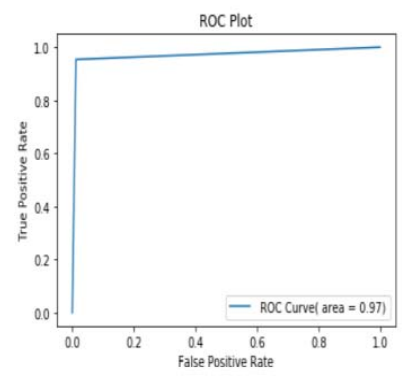
\includegraphics[width=1\textwidth]{Roc bagging.png}
	\end{minipage}}
\end{figure}
ROC plot of Logistic Regression  obtained 95\% score. Highest ROC scores 97\% is obtained for XGBoost 
and Bagging classifier.
\end{block}
\end{frame}
\begin{frame}
\begin{block}{Precision-recall plot}
\begin{figure}[ht]
  \subfloat[\scriptsize{logistic regression}]{
	\begin{minipage}[c][1\width]{
	   0.3\textwidth}
	   \centering
	   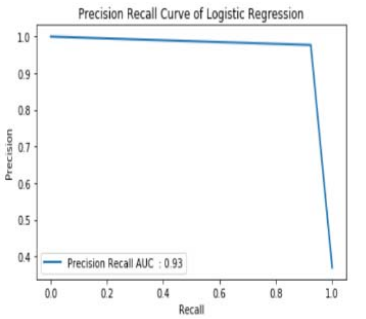
\includegraphics[width=1\textwidth]{precision plot logistic.png}
	\end{minipage}}
 \hfill 	
  \subfloat[\scriptsize{XGBoost}]{
	\begin{minipage}[c][1\width]{
	   0.3\textwidth}
	   \centering
	   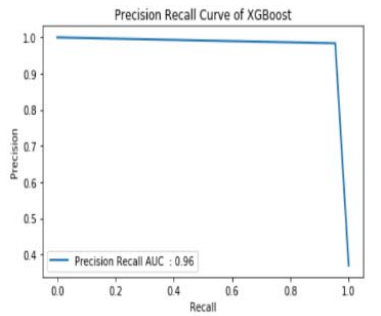
\includegraphics[width=1\textwidth]{precision plot XGBoost.png}
	\end{minipage}}
 \hfill	
  \subfloat[\scriptsize{bagging}]{
	\begin{minipage}[c][1\width]{
	   0.3\textwidth}
	   \centering
	   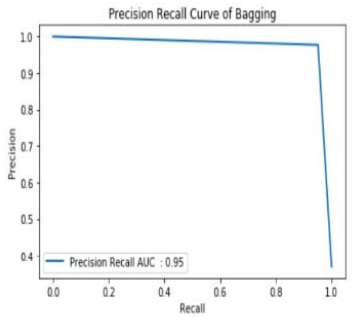
\includegraphics[width=1\textwidth]{precision plot bagging.png}
	\end{minipage}}
\end{figure}
Precision-Recall plot for logistic regression is obtained 93\% 
,and 95\% as been achieved by Bagging classifier.XGBoost has obtained the highest Precision recall score as 96\%.
\end{block}
\end{frame}
\begin{frame}
\begin{block}{Summing up}
After plotting all plots and Precision,recall,F1-score,accuracy are calculated and tabulated as shown below.
\begin{figure}[ht]
    \centering
    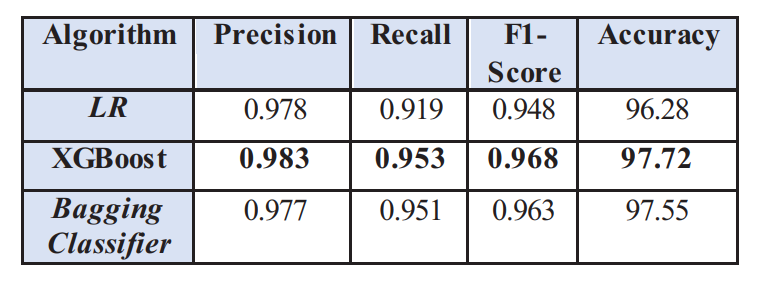
\includegraphics[width =0.7
    \columnwidth]{experiment precision recall.png}
\end{figure}
From all the evaluation highest score is obtained for the XGBoost algorithm when compared to others it has an highest accuracy of \textbf{97.7\%}.Hence XG boost is the best algorithm for recommending users based on link prediction techinique.
\end{block}
\end{frame}
\begin{frame}{CONCLUSION}
\begin{block}{}
Many unsupervised link prediction features are implemented and  suitable features are chosen using chi-square test .Here from the experimental results we can see that Among Logistic Regression, XGboost and Bagging Classifier.XGBoost has obtained a good score in all the performance  measures and obtained the highest accuracy of 97.72\% compared to other implementation.Hence XGBoost is the most preferrable for building the model.
\end{block}
\end{frame}
\begin{frame}
     \centering
    \textcolor{blue}{\Huge{\textbf{THANK YOU}}}
\end{frame}
\end{document}